% Created by tikzDevice version 0.10.1 on 2016-06-26 23:09:38
% !TEX encoding = UTF-8 Unicode
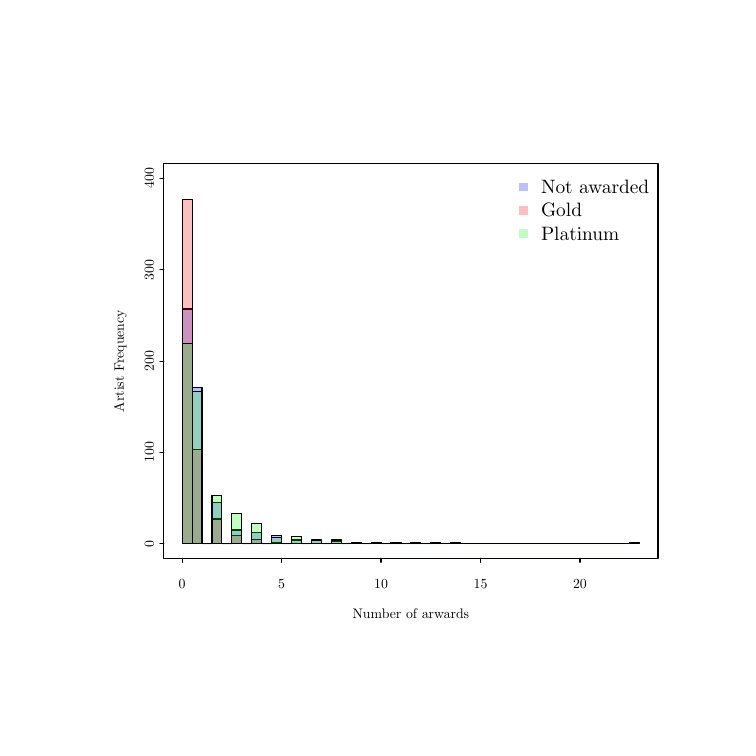
\begin{tikzpicture}[x=1pt,y=1pt]
\definecolor{fillColor}{RGB}{255,255,255}
\path[use as bounding box,fill=fillColor,fill opacity=0.00] (0,0) rectangle (252.94,252.94);
\begin{scope}
\path[clip] (  0.00,  0.00) rectangle (252.94,252.94);
\definecolor{drawColor}{RGB}{0,0,0}

\node[text=drawColor,anchor=base,inner sep=0pt, outer sep=0pt, scale=  0.50] at (138.47, 39.60) {Number of arwards};

\node[text=drawColor,rotate= 90.00,anchor=base,inner sep=0pt, outer sep=0pt, scale=  0.50] at ( 34.80,132.47) {Artist Frequency};
\end{scope}
\begin{scope}
\path[clip] (  0.00,  0.00) rectangle (252.94,252.94);
\definecolor{drawColor}{RGB}{0,0,0}

\path[draw=drawColor,line width= 0.4pt,line join=round,line cap=round] ( 55.81, 61.20) -- (199.57, 61.20);

\path[draw=drawColor,line width= 0.4pt,line join=round,line cap=round] ( 55.81, 61.20) -- ( 55.81, 59.77);

\path[draw=drawColor,line width= 0.4pt,line join=round,line cap=round] ( 91.75, 61.20) -- ( 91.75, 59.77);

\path[draw=drawColor,line width= 0.4pt,line join=round,line cap=round] (127.69, 61.20) -- (127.69, 59.77);

\path[draw=drawColor,line width= 0.4pt,line join=round,line cap=round] (163.63, 61.20) -- (163.63, 59.77);

\path[draw=drawColor,line width= 0.4pt,line join=round,line cap=round] (199.57, 61.20) -- (199.57, 59.77);

\node[text=drawColor,anchor=base,inner sep=0pt, outer sep=0pt, scale=  0.50] at ( 55.81, 50.40) {0};

\node[text=drawColor,anchor=base,inner sep=0pt, outer sep=0pt, scale=  0.50] at ( 91.75, 50.40) {5};

\node[text=drawColor,anchor=base,inner sep=0pt, outer sep=0pt, scale=  0.50] at (127.69, 50.40) {10};

\node[text=drawColor,anchor=base,inner sep=0pt, outer sep=0pt, scale=  0.50] at (163.63, 50.40) {15};

\node[text=drawColor,anchor=base,inner sep=0pt, outer sep=0pt, scale=  0.50] at (199.57, 50.40) {20};

\path[draw=drawColor,line width= 0.4pt,line join=round,line cap=round] ( 49.20, 66.48) -- ( 49.20,198.47);

\path[draw=drawColor,line width= 0.4pt,line join=round,line cap=round] ( 49.20, 66.48) -- ( 47.77, 66.48);

\path[draw=drawColor,line width= 0.4pt,line join=round,line cap=round] ( 49.20, 99.48) -- ( 47.77, 99.48);

\path[draw=drawColor,line width= 0.4pt,line join=round,line cap=round] ( 49.20,132.47) -- ( 47.77,132.47);

\path[draw=drawColor,line width= 0.4pt,line join=round,line cap=round] ( 49.20,165.47) -- ( 47.77,165.47);

\path[draw=drawColor,line width= 0.4pt,line join=round,line cap=round] ( 49.20,198.47) -- ( 47.77,198.47);

\node[text=drawColor,rotate= 90.00,anchor=base,inner sep=0pt, outer sep=0pt, scale=  0.50] at ( 45.60, 66.48) {0};

\node[text=drawColor,rotate= 90.00,anchor=base,inner sep=0pt, outer sep=0pt, scale=  0.50] at ( 45.60, 99.48) {100};

\node[text=drawColor,rotate= 90.00,anchor=base,inner sep=0pt, outer sep=0pt, scale=  0.50] at ( 45.60,132.47) {200};

\node[text=drawColor,rotate= 90.00,anchor=base,inner sep=0pt, outer sep=0pt, scale=  0.50] at ( 45.60,165.47) {300};

\node[text=drawColor,rotate= 90.00,anchor=base,inner sep=0pt, outer sep=0pt, scale=  0.50] at ( 45.60,198.47) {400};
\end{scope}
\begin{scope}
\path[clip] ( 49.20, 61.20) rectangle (227.75,203.75);
\definecolor{drawColor}{RGB}{0,0,0}
\definecolor{fillColor}{RGB}{0,0,255}

\path[draw=drawColor,line width= 0.4pt,line join=round,line cap=round,fill=fillColor,fill opacity=0.25] ( 55.81, 66.48) rectangle ( 59.41,151.28);

\path[draw=drawColor,line width= 0.4pt,line join=round,line cap=round,fill=fillColor,fill opacity=0.25] ( 59.41, 66.48) rectangle ( 63.00,122.90);

\path[draw=drawColor,line width= 0.4pt,line join=round,line cap=round,fill=fillColor,fill opacity=0.25] ( 63.00, 66.48) rectangle ( 66.59, 66.48);

\path[draw=drawColor,line width= 0.4pt,line join=round,line cap=round,fill=fillColor,fill opacity=0.25] ( 66.59, 66.48) rectangle ( 70.19, 81.33);

\path[draw=drawColor,line width= 0.4pt,line join=round,line cap=round,fill=fillColor,fill opacity=0.25] ( 70.19, 66.48) rectangle ( 73.78, 66.48);

\path[draw=drawColor,line width= 0.4pt,line join=round,line cap=round,fill=fillColor,fill opacity=0.25] ( 73.78, 66.48) rectangle ( 77.38, 71.43);

\path[draw=drawColor,line width= 0.4pt,line join=round,line cap=round,fill=fillColor,fill opacity=0.25] ( 77.38, 66.48) rectangle ( 80.97, 66.48);

\path[draw=drawColor,line width= 0.4pt,line join=round,line cap=round,fill=fillColor,fill opacity=0.25] ( 80.97, 66.48) rectangle ( 84.56, 70.44);

\path[draw=drawColor,line width= 0.4pt,line join=round,line cap=round,fill=fillColor,fill opacity=0.25] ( 84.56, 66.48) rectangle ( 88.16, 66.48);

\path[draw=drawColor,line width= 0.4pt,line join=round,line cap=round,fill=fillColor,fill opacity=0.25] ( 88.16, 66.48) rectangle ( 91.75, 69.45);

\path[draw=drawColor,line width= 0.4pt,line join=round,line cap=round,fill=fillColor,fill opacity=0.25] ( 91.75, 66.48) rectangle ( 95.35, 66.48);

\path[draw=drawColor,line width= 0.4pt,line join=round,line cap=round,fill=fillColor,fill opacity=0.25] ( 95.35, 66.48) rectangle ( 98.94, 67.80);

\path[draw=drawColor,line width= 0.4pt,line join=round,line cap=round,fill=fillColor,fill opacity=0.25] ( 98.94, 66.48) rectangle (102.53, 66.48);

\path[draw=drawColor,line width= 0.4pt,line join=round,line cap=round,fill=fillColor,fill opacity=0.25] (102.53, 66.48) rectangle (106.13, 67.80);

\path[draw=drawColor,line width= 0.4pt,line join=round,line cap=round,fill=fillColor,fill opacity=0.25] (106.13, 66.48) rectangle (109.72, 66.48);

\path[draw=drawColor,line width= 0.4pt,line join=round,line cap=round,fill=fillColor,fill opacity=0.25] (109.72, 66.48) rectangle (113.32, 67.14);

\path[draw=drawColor,line width= 0.4pt,line join=round,line cap=round,fill=fillColor,fill opacity=0.25] (113.32, 66.48) rectangle (116.91, 66.48);

\path[draw=drawColor,line width= 0.4pt,line join=round,line cap=round,fill=fillColor,fill opacity=0.25] (116.91, 66.48) rectangle (120.50, 66.81);

\path[draw=drawColor,line width= 0.4pt,line join=round,line cap=round,fill=fillColor,fill opacity=0.25] (120.50, 66.48) rectangle (124.10, 66.48);

\path[draw=drawColor,line width= 0.4pt,line join=round,line cap=round,fill=fillColor,fill opacity=0.25] (124.10, 66.48) rectangle (127.69, 66.81);

\path[draw=drawColor,line width= 0.4pt,line join=round,line cap=round,fill=fillColor,fill opacity=0.25] (127.69, 66.48) rectangle (131.28, 66.48);

\path[draw=drawColor,line width= 0.4pt,line join=round,line cap=round,fill=fillColor,fill opacity=0.25] (131.28, 66.48) rectangle (134.88, 66.48);

\path[draw=drawColor,line width= 0.4pt,line join=round,line cap=round,fill=fillColor,fill opacity=0.25] (134.88, 66.48) rectangle (138.47, 66.48);

\path[draw=drawColor,line width= 0.4pt,line join=round,line cap=round,fill=fillColor,fill opacity=0.25] (138.47, 66.48) rectangle (142.07, 66.48);

\path[draw=drawColor,line width= 0.4pt,line join=round,line cap=round,fill=fillColor,fill opacity=0.25] (142.07, 66.48) rectangle (145.66, 66.48);

\path[draw=drawColor,line width= 0.4pt,line join=round,line cap=round,fill=fillColor,fill opacity=0.25] (145.66, 66.48) rectangle (149.25, 66.81);
\definecolor{fillColor}{RGB}{255,0,0}

\path[draw=drawColor,line width= 0.4pt,line join=round,line cap=round,fill=fillColor,fill opacity=0.25] ( 55.81, 66.48) rectangle ( 59.41,190.88);

\path[draw=drawColor,line width= 0.4pt,line join=round,line cap=round,fill=fillColor,fill opacity=0.25] ( 59.41, 66.48) rectangle ( 63.00,100.47);

\path[draw=drawColor,line width= 0.4pt,line join=round,line cap=round,fill=fillColor,fill opacity=0.25] ( 63.00, 66.48) rectangle ( 66.59, 66.48);

\path[draw=drawColor,line width= 0.4pt,line join=round,line cap=round,fill=fillColor,fill opacity=0.25] ( 66.59, 66.48) rectangle ( 70.19, 75.39);

\path[draw=drawColor,line width= 0.4pt,line join=round,line cap=round,fill=fillColor,fill opacity=0.25] ( 70.19, 66.48) rectangle ( 73.78, 66.48);

\path[draw=drawColor,line width= 0.4pt,line join=round,line cap=round,fill=fillColor,fill opacity=0.25] ( 73.78, 66.48) rectangle ( 77.38, 69.45);

\path[draw=drawColor,line width= 0.4pt,line join=round,line cap=round,fill=fillColor,fill opacity=0.25] ( 77.38, 66.48) rectangle ( 80.97, 66.48);

\path[draw=drawColor,line width= 0.4pt,line join=round,line cap=round,fill=fillColor,fill opacity=0.25] ( 80.97, 66.48) rectangle ( 84.56, 68.13);

\path[draw=drawColor,line width= 0.4pt,line join=round,line cap=round,fill=fillColor,fill opacity=0.25] ( 84.56, 66.48) rectangle ( 88.16, 66.48);

\path[draw=drawColor,line width= 0.4pt,line join=round,line cap=round,fill=fillColor,fill opacity=0.25] ( 88.16, 66.48) rectangle ( 91.75, 66.81);
\definecolor{fillColor}{RGB}{0,255,0}

\path[draw=drawColor,line width= 0.4pt,line join=round,line cap=round,fill=fillColor,fill opacity=0.25] ( 55.81, 66.48) rectangle ( 59.41,138.74);

\path[draw=drawColor,line width= 0.4pt,line join=round,line cap=round,fill=fillColor,fill opacity=0.25] ( 59.41, 66.48) rectangle ( 63.00,121.58);

\path[draw=drawColor,line width= 0.4pt,line join=round,line cap=round,fill=fillColor,fill opacity=0.25] ( 63.00, 66.48) rectangle ( 66.59, 66.48);

\path[draw=drawColor,line width= 0.4pt,line join=round,line cap=round,fill=fillColor,fill opacity=0.25] ( 66.59, 66.48) rectangle ( 70.19, 83.97);

\path[draw=drawColor,line width= 0.4pt,line join=round,line cap=round,fill=fillColor,fill opacity=0.25] ( 70.19, 66.48) rectangle ( 73.78, 66.48);

\path[draw=drawColor,line width= 0.4pt,line join=round,line cap=round,fill=fillColor,fill opacity=0.25] ( 73.78, 66.48) rectangle ( 77.38, 77.37);

\path[draw=drawColor,line width= 0.4pt,line join=round,line cap=round,fill=fillColor,fill opacity=0.25] ( 77.38, 66.48) rectangle ( 80.97, 66.48);

\path[draw=drawColor,line width= 0.4pt,line join=round,line cap=round,fill=fillColor,fill opacity=0.25] ( 80.97, 66.48) rectangle ( 84.56, 73.74);

\path[draw=drawColor,line width= 0.4pt,line join=round,line cap=round,fill=fillColor,fill opacity=0.25] ( 84.56, 66.48) rectangle ( 88.16, 66.48);

\path[draw=drawColor,line width= 0.4pt,line join=round,line cap=round,fill=fillColor,fill opacity=0.25] ( 88.16, 66.48) rectangle ( 91.75, 68.79);

\path[draw=drawColor,line width= 0.4pt,line join=round,line cap=round,fill=fillColor,fill opacity=0.25] ( 91.75, 66.48) rectangle ( 95.35, 66.48);

\path[draw=drawColor,line width= 0.4pt,line join=round,line cap=round,fill=fillColor,fill opacity=0.25] ( 95.35, 66.48) rectangle ( 98.94, 69.12);

\path[draw=drawColor,line width= 0.4pt,line join=round,line cap=round,fill=fillColor,fill opacity=0.25] ( 98.94, 66.48) rectangle (102.53, 66.48);

\path[draw=drawColor,line width= 0.4pt,line join=round,line cap=round,fill=fillColor,fill opacity=0.25] (102.53, 66.48) rectangle (106.13, 67.47);

\path[draw=drawColor,line width= 0.4pt,line join=round,line cap=round,fill=fillColor,fill opacity=0.25] (106.13, 66.48) rectangle (109.72, 66.48);

\path[draw=drawColor,line width= 0.4pt,line join=round,line cap=round,fill=fillColor,fill opacity=0.25] (109.72, 66.48) rectangle (113.32, 67.80);

\path[draw=drawColor,line width= 0.4pt,line join=round,line cap=round,fill=fillColor,fill opacity=0.25] (113.32, 66.48) rectangle (116.91, 66.48);

\path[draw=drawColor,line width= 0.4pt,line join=round,line cap=round,fill=fillColor,fill opacity=0.25] (116.91, 66.48) rectangle (120.50, 66.81);

\path[draw=drawColor,line width= 0.4pt,line join=round,line cap=round,fill=fillColor,fill opacity=0.25] (120.50, 66.48) rectangle (124.10, 66.48);

\path[draw=drawColor,line width= 0.4pt,line join=round,line cap=round,fill=fillColor,fill opacity=0.25] (124.10, 66.48) rectangle (127.69, 66.81);

\path[draw=drawColor,line width= 0.4pt,line join=round,line cap=round,fill=fillColor,fill opacity=0.25] (127.69, 66.48) rectangle (131.28, 66.48);

\path[draw=drawColor,line width= 0.4pt,line join=round,line cap=round,fill=fillColor,fill opacity=0.25] (131.28, 66.48) rectangle (134.88, 66.81);

\path[draw=drawColor,line width= 0.4pt,line join=round,line cap=round,fill=fillColor,fill opacity=0.25] (134.88, 66.48) rectangle (138.47, 66.48);

\path[draw=drawColor,line width= 0.4pt,line join=round,line cap=round,fill=fillColor,fill opacity=0.25] (138.47, 66.48) rectangle (142.07, 66.81);

\path[draw=drawColor,line width= 0.4pt,line join=round,line cap=round,fill=fillColor,fill opacity=0.25] (142.07, 66.48) rectangle (145.66, 66.48);

\path[draw=drawColor,line width= 0.4pt,line join=round,line cap=round,fill=fillColor,fill opacity=0.25] (145.66, 66.48) rectangle (149.25, 66.48);

\path[draw=drawColor,line width= 0.4pt,line join=round,line cap=round,fill=fillColor,fill opacity=0.25] (149.25, 66.48) rectangle (152.85, 66.48);

\path[draw=drawColor,line width= 0.4pt,line join=round,line cap=round,fill=fillColor,fill opacity=0.25] (152.85, 66.48) rectangle (156.44, 66.81);

\path[draw=drawColor,line width= 0.4pt,line join=round,line cap=round,fill=fillColor,fill opacity=0.25] (156.44, 66.48) rectangle (160.04, 66.48);

\path[draw=drawColor,line width= 0.4pt,line join=round,line cap=round,fill=fillColor,fill opacity=0.25] (160.04, 66.48) rectangle (163.63, 66.48);

\path[draw=drawColor,line width= 0.4pt,line join=round,line cap=round,fill=fillColor,fill opacity=0.25] (163.63, 66.48) rectangle (167.22, 66.48);

\path[draw=drawColor,line width= 0.4pt,line join=round,line cap=round,fill=fillColor,fill opacity=0.25] (167.22, 66.48) rectangle (170.82, 66.48);

\path[draw=drawColor,line width= 0.4pt,line join=round,line cap=round,fill=fillColor,fill opacity=0.25] (170.82, 66.48) rectangle (174.41, 66.48);

\path[draw=drawColor,line width= 0.4pt,line join=round,line cap=round,fill=fillColor,fill opacity=0.25] (174.41, 66.48) rectangle (178.01, 66.48);

\path[draw=drawColor,line width= 0.4pt,line join=round,line cap=round,fill=fillColor,fill opacity=0.25] (178.01, 66.48) rectangle (181.60, 66.48);

\path[draw=drawColor,line width= 0.4pt,line join=round,line cap=round,fill=fillColor,fill opacity=0.25] (181.60, 66.48) rectangle (185.19, 66.48);

\path[draw=drawColor,line width= 0.4pt,line join=round,line cap=round,fill=fillColor,fill opacity=0.25] (185.19, 66.48) rectangle (188.79, 66.48);

\path[draw=drawColor,line width= 0.4pt,line join=round,line cap=round,fill=fillColor,fill opacity=0.25] (188.79, 66.48) rectangle (192.38, 66.48);

\path[draw=drawColor,line width= 0.4pt,line join=round,line cap=round,fill=fillColor,fill opacity=0.25] (192.38, 66.48) rectangle (195.97, 66.48);

\path[draw=drawColor,line width= 0.4pt,line join=round,line cap=round,fill=fillColor,fill opacity=0.25] (195.97, 66.48) rectangle (199.57, 66.48);

\path[draw=drawColor,line width= 0.4pt,line join=round,line cap=round,fill=fillColor,fill opacity=0.25] (199.57, 66.48) rectangle (203.16, 66.48);

\path[draw=drawColor,line width= 0.4pt,line join=round,line cap=round,fill=fillColor,fill opacity=0.25] (203.16, 66.48) rectangle (206.76, 66.48);

\path[draw=drawColor,line width= 0.4pt,line join=round,line cap=round,fill=fillColor,fill opacity=0.25] (206.76, 66.48) rectangle (210.35, 66.48);

\path[draw=drawColor,line width= 0.4pt,line join=round,line cap=round,fill=fillColor,fill opacity=0.25] (210.35, 66.48) rectangle (213.94, 66.48);

\path[draw=drawColor,line width= 0.4pt,line join=round,line cap=round,fill=fillColor,fill opacity=0.25] (213.94, 66.48) rectangle (217.54, 66.48);

\path[draw=drawColor,line width= 0.4pt,line join=round,line cap=round,fill=fillColor,fill opacity=0.25] (217.54, 66.48) rectangle (221.13, 66.81);
\definecolor{fillColor}{RGB}{0,0,255}

\path[fill=fillColor,fill opacity=0.25] (177.63,193.77) --
	(180.78,193.77) --
	(180.78,196.92) --
	(177.63,196.92) --
	cycle;
\definecolor{fillColor}{RGB}{255,0,0}

\path[fill=fillColor,fill opacity=0.25] (177.63,185.37) --
	(180.78,185.37) --
	(180.78,188.52) --
	(177.63,188.52) --
	cycle;
\definecolor{fillColor}{RGB}{0,255,0}

\path[fill=fillColor,fill opacity=0.25] (177.63,176.97) --
	(180.78,176.97) --
	(180.78,180.12) --
	(177.63,180.12) --
	cycle;

\node[text=drawColor,anchor=base west,inner sep=0pt, outer sep=0pt, scale=  0.70] at (185.50,192.93) {Not awarded};

\node[text=drawColor,anchor=base west,inner sep=0pt, outer sep=0pt, scale=  0.70] at (185.50,184.53) {Gold};

\node[text=drawColor,anchor=base west,inner sep=0pt, outer sep=0pt, scale=  0.70] at (185.50,176.13) {Platinum};
\end{scope}
\begin{scope}
\path[clip] (  0.00,  0.00) rectangle (252.94,252.94);
\definecolor{drawColor}{RGB}{0,0,0}

\path[draw=drawColor,line width= 0.4pt,line join=round,line cap=round] ( 49.20, 61.20) --
	(227.75, 61.20) --
	(227.75,203.75) --
	( 49.20,203.75) --
	( 49.20, 61.20);
\end{scope}
\end{tikzpicture}
